% !TEX program = lualatex
\documentclass[aspectratio=43,professionalfonts,handout]{beamer}
\usepackage{beamer_template}

\newcommand{\LectureNum}{13}
\newcommand{\LectureTitle}{余弦定理・三角形の面積}
\newcommand{\TextPages}{p.\,135-137}
\newcommand{\NextTopic}{三角形への応用（総合演習）}
\newcommand{\NextPages}{p.\,138-139（練習問題1-A, 1-B）}
\newcommand{\CourseName}{基礎数学B}
\renewcommand{\TermName}{後期}

\begin{document}

% -----------------------------------------------
% スライド1: 表紙＋目標＋用語・定義
% -----------------------------------------------
\begin{frame}{\CourseName\quad 第\LectureNum 回「\LectureTitle 」}
  {\small \TermName\quad \TeacherName\quad ／\quad 教科書 \TextPages\quad
  \textbf{目標}：余弦定理を用いて辺と角を求め、面積公式を使える}

  \begin{block}{用語・定義}
  \begin{description}[labelwidth=5.5em]
    \item[\kw{余弦定理：a²=b²+c²-2bc cosA}] ~
    \item[\kw{面積公式：S=½bc sinA}] ~
    \item[\kw{ヘロンの公式}] ~
  \end{description}
  \end{block}
\end{frame}

% -----------------------------------------------
% スライド2: 公式・性質
% -----------------------------------------------
\begin{frame}{公式・性質}
  \begin{block}{}
  \begin{itemize}
    \item 余弦定理の2つの使い方：辺を求める・角を求める
    \item S=½bc sinA から角を求める逆算
    \item ヘロン：s=(a+b+c)/2、S=√(s(s-a)(s-b)(s-c))
  \end{itemize}
  \end{block}
\end{frame}

% -----------------------------------------------
% スライド3: 図・グラフ（TikZコードを手動追加）
% -----------------------------------------------
\begin{frame}{図・グラフ}
  \centering
  % TODO: 余弦定理の幾何的意味（ピタゴラスの拡張）
  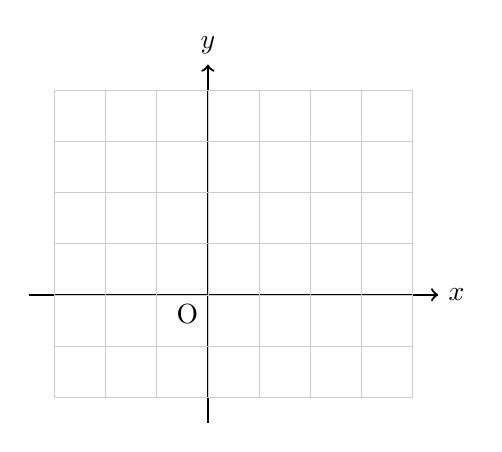
\begin{tikzpicture}[scale=0.65]
    \draw[->,thick] (-3.5,0) -- (4.5,0) node[right]{$x$};
    \draw[->,thick] (0,-2.5) -- (0,4.5) node[above]{$y$};
    \node[below left] at (0,0) {O};
    \draw[gray!40, very thin] (-3,-2) grid (4,4);
    % ここにグラフを描画
  \end{tikzpicture}
\end{frame}

% -----------------------------------------------
% スライド4: 例1→問1
% -----------------------------------------------
\begin{frame}{例1→問1}
  \begin{exampleblock}{例題3) p.140（余弦定理で辺・角を求める）}
    （板書で解説）
  \end{exampleblock}

  \vfill

  \begin{block}{問5) p.140\quad 自分で解いてみよう}
    （ノートに解くこと）
  \end{block}
\end{frame}

% -----------------------------------------------
% スライド5: 例2→問2
% -----------------------------------------------
\begin{frame}{例2→問2}
  \begin{exampleblock}{例題4) p.141（面積・ヘロン）}
    （板書で解説）
  \end{exampleblock}

  \vfill

  \begin{block}{問6) p.141\quad 自分で解いてみよう}
    （ノートに解くこと）
  \end{block}
\end{frame}

% -----------------------------------------------
% まとめ
% -----------------------------------------------
\begin{frame}{まとめ}
  \begin{itemize}
    \item % TODO: まとめを記入
  \end{itemize}

  \vfill
  {\small 基本問題：266, 267, 268, 269, 270, 271}
\end{frame}

\end{document}
